
\lettrine[lines=3]{T}{}he string interpreter is one of the significant components of plant generation. It is the final step in the process of procedural generation. The output of this stage is dependant on what the L-system is representing. In this case, it is responsible for creating the final plant models and other information and then rendering it on the screen, using the OpenGL framework. 

The interpreter has three main stages of processing, which can be seen in figure \ref{l-system interpreter}. The first part is the turtle graphics interpreter, then the model generator, and finally, the renderer. The turtle graphics interpreter takes the string of modules provided by the rewriter, as a set of instructions. It starts from the root of the tree and generates a skeletal structure made up of joints. This is similar to the techniques used in skeletal rigging in animation \cite{gregory2014game}. The tree skeleton joints each represent a branch segment or part of the tree. These joints have some information about the properties of that segment. The joint data is not only used to generate the model data but also to make it simpler to do physics calculations. The model generator creates the points that make up the plant in 3D space, as well as calculating the texture and lighting information. The models can finally be passed to the renderer. The renderer is responsible for taking all the model information such as, vertex, texture, and lighting data and renders the final plant on the screen. 

This chapter will firstly focus on the use of a skeletal structure to represent plant-life, and why this is useful in the plant model generation and simulation of motion. It will then discuss the details of how the plant skeleton is created using the L-system instructions and turtle graphics interpreter. The details of model generation will be discussed focusing on two straightforward techniques of modeling the branching structure. Finally it will breifly discuss how the information can be used to render the model on the screen. It is important to note that the model generator and renderer implementation are reasonably straight forward as they are not the focus of this thesis. It is possible to generate very intricate and hightly complex rendering systems that will further improve the look of the plants, however, the skeletal structure and basic model generation concepts will remain the same.

\begin{figure}[htbp]
	{\centering
		\vspace{7px}
		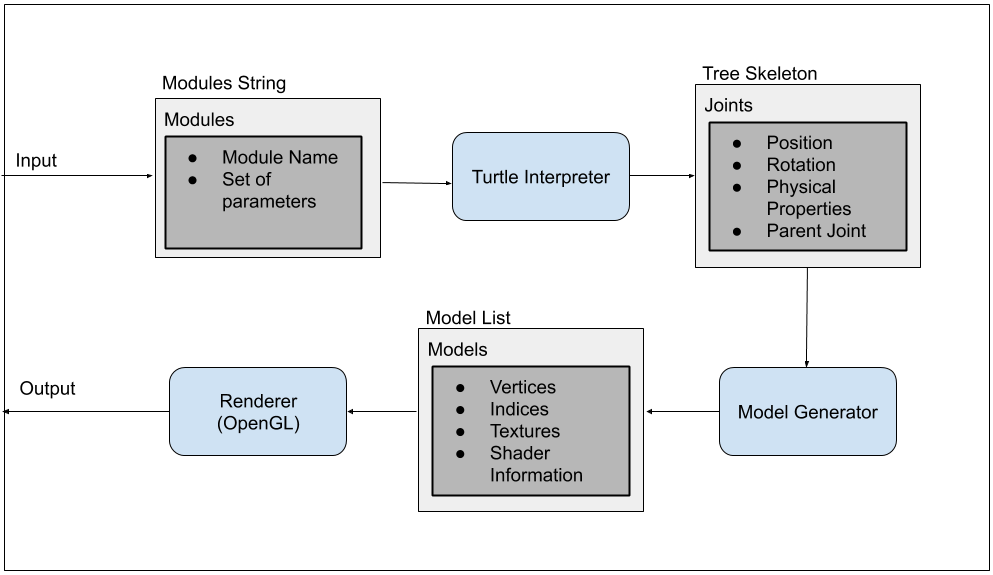
\includegraphics[scale=0.4]{Diagrams/L-systemInterpreter.png}
		\caption{Diagram of the three stages of L-system interpretation} \label{l-system interpreter}
	}
\end{figure}
\FloatBarrier

\section{Turtle Graphics Interpreter} \label{turtle graphics section}

The primary purpose of the turtle graphics interpreter is to take the string of modules from the L-system rewriter and interpret each module as a turtle graphics instruction. Each instruction carries out a particular job in creating the overall structure of the plant. This stage is purely to follow the turtle graphics instructions and generate the skeletal data of the plant for the next stage.

The process of skeletal rigging is often used within 3D graphics in character design in order to make characters able to move. This process takes several joints and links them to various movable parts of the body. The joints are often linked together by a central joint known as the pelvis joint, as it is in the pelvis of the character being rigged. The joints are linked in a hierarchy such that moving a parent joint will affect all of the child joints. For instance, moving a character's elbow would, in turn, move its wrist, hand, and fingers. This same concept can be used for plants. The L-system creates the instructions for a tree that is made up of branch segments. Each branch segment is a joint in the larger plant skeleton. Instead of a pelvis joint, the plant will have a root joint, being the joint at the very root of the plant. 

The figure in \ref{skeleton diagram} below shows how the plant structure can be broken down into a skeleton. In this case, Joint 0 is the root joint. For areas where the plant branches in two or more directions, a joint is needed to represent each branch segment, and therefore there are two joints in a single position. The resulting string of modules that is used to build this structure is: \\
\\
F(3)[+(25)!(2.5)F(3)[+(25)!(1.0)F(3)]-(25)F(3)]\&(25)!(2.5)F(3)[\&(25)!(1)F(3)]-(25)!(1)F(3);

\begin{figure}[htbp]
	{\centering
		\vspace{7px}
		\setlength{\fboxrule}{1pt}
		\fbox{
			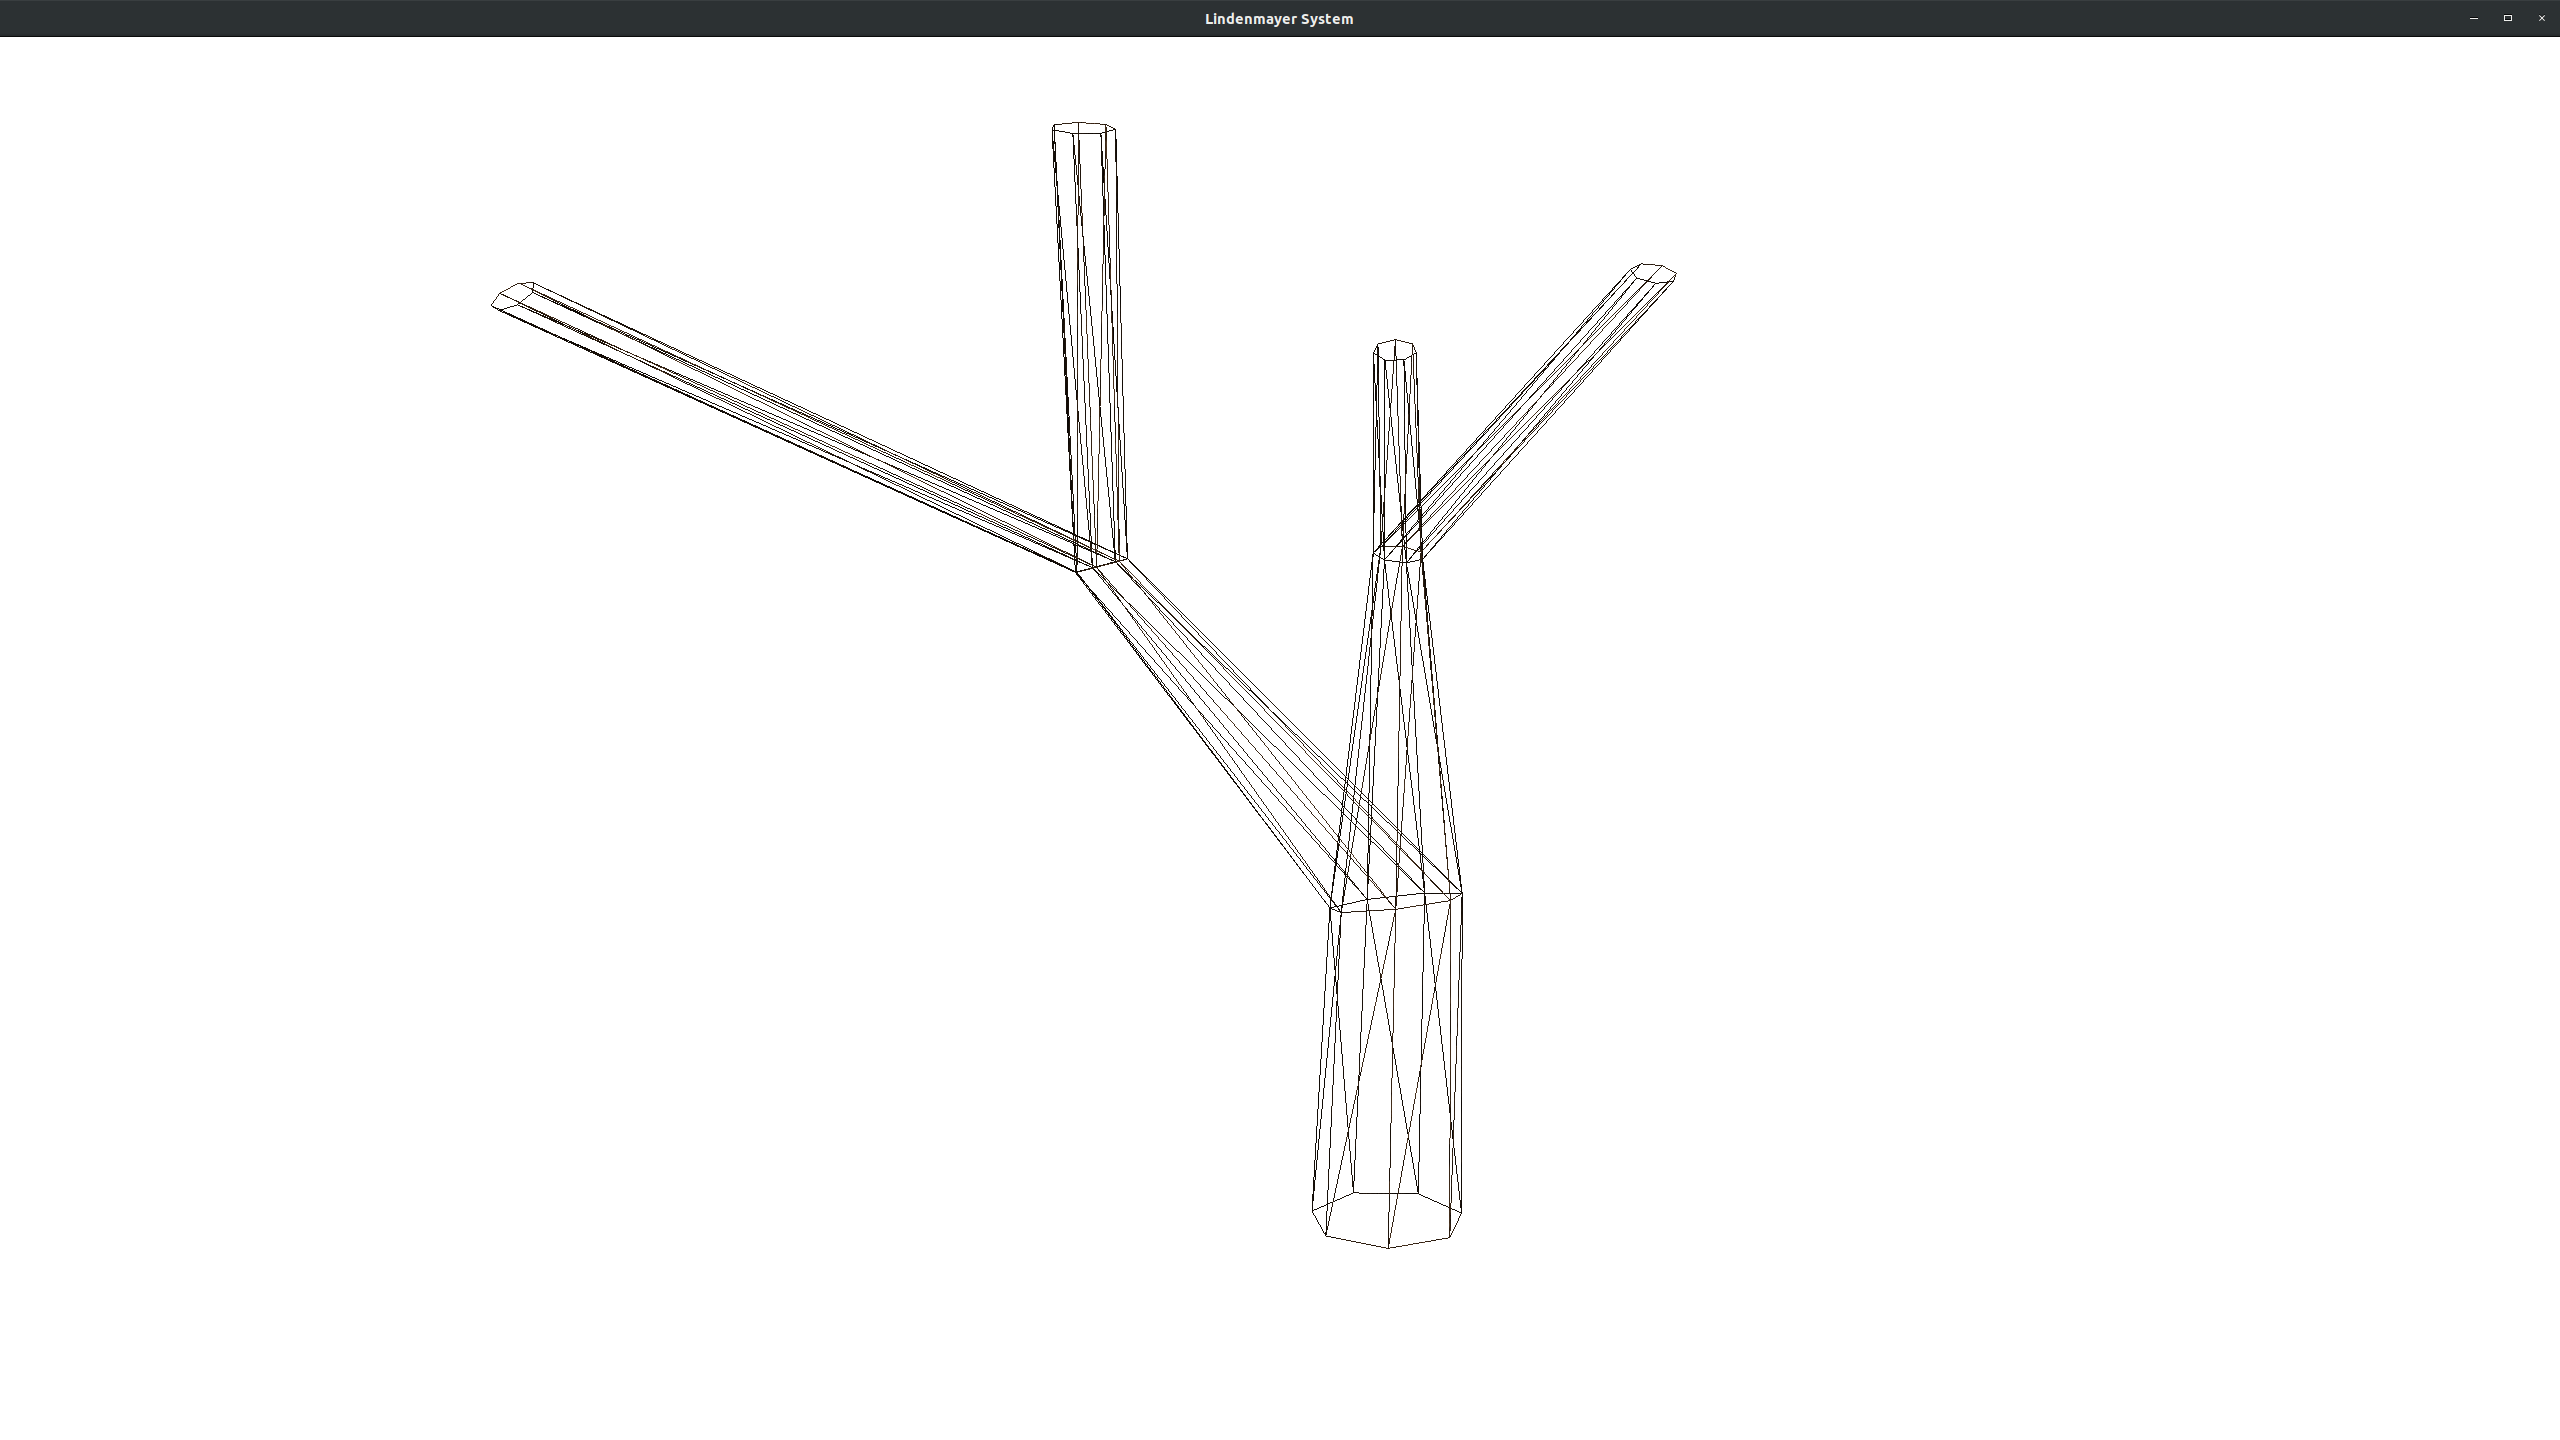
\includegraphics[scale=0.20]{Diagrams/treeSkeleton.png}
		}
		\caption{Diagram of a simple plant skeleton showing the joint positions.} \label{skeleton diagram}
	}
\end{figure}
\FloatBarrier

\noindent
Through the process of turtle graphics interpretation, each joint can be created and added to the skeleton. This process will be talked about in more detail later in this section. However, it is essential first to discuss the properties of each joint and its importance.

Figure \ref{joint properties} shows the information stored for each joint within the skeleton. There is a large amount of information stored for the position and orientation of each joint. This is because the rotation of the joint is stored in both a local and global space. Local space refers to the joint's rotation relative to its parent rotation. This is useful as it allows the manipulation of subsequent child joints while leaving other joints local rotation unchanged. Global space, also known as world space, is the rotation of each joint relative to the world itself. This is useful for understanding the current rotation of the joint relative to the world. It is essential to store both the current and previous rotations as they are used to calculate the rate of change for physics calculations.

The physical properties for each joint are the parts that will affect model generation as well as physics simulations. These properties include the length, width, spring constant, damping constant as well as the current momentum of the branch.

\begin{figure}[htbp]
	{\centering
		\vspace{7px}
		\setlength{\fboxrule}{1pt}
		\fbox{
			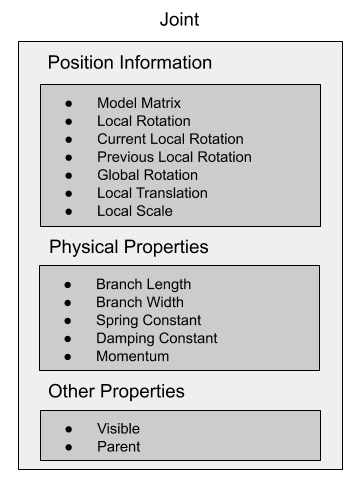
\includegraphics[scale=0.6]{Diagrams/JointDiagram.png}
		}
		\caption{Diagram for the properties of a joint} \label{joint properties}
	}
\end{figure}
\FloatBarrier

\noindent
The skeletal structure of the plant must be created by interpreting the result string of the L-system rewriter. In essence, this interpreter is a more sophisticated version of the implementation that was covered in section \ref{Interpreting DOL-system} of the DOL-system interpreter. The main difference between these interpreters is that the L-system string is produced by a parametric L-system and, therefore, consists of modules and parameters instead of characters. Despite these differences, the overall concept remains the same. Each module name within the L-systems resultant string represents a particular meaning to the turtle graphics interpreter. The meaning of the module names are predefined in the string interpreter system and are dependant on what the L-system is trying to represent. The L-system defined for this thesis allows each module to provide optional parameters. These parameters may also carry particular meanings for the interpreter. For instance, the forward instruction or module name \say{F} can have two parameters. The value of the first parameter is the distance to move forward. The second parameter is the spring constant of the branch. If these parameters are not provided, then a default value will be used. 

Below is a table describing the L-system module names as well as the parameter meanings for the turtle graphics interpreter. In all of the instructions, there is also the case where no parameter is provided. This is still valid; however, if no parameter value is provided, a default value will be used.

\begin{table}[h!]
\centering
\begin{tabular}{ | c | l | l | l |}
\hline
	Instruction Name  & Meaning					& Parameter 1 	& Parameter 2 					\\  
\hline
\hline
	F 				&	Forward (Render)		& Length		& Spring Constant				\\
\hline
	f 				&	Forward (Don't render)	& Length 		& Spring Constant				\\
\hline
	+ 				&	Yaw	Right				& Angle 		&	N/A							\\
\hline
	- 				&	Yaw Left				& Angle			&	N/A							\\
\hline
	/ 				&	Pitch Up				& Angle			&	N/A							\\
\hline
	$\backslash$ 	&	Pitch Down				& Angle			&	N/A							\\
\hline
	$\land$ 		&	Roll Right				& Angle			&	N/A							\\
\hline
	\& 				&	Roll Left				& Angle 		&	N/A							\\
\hline
	! 				&	Change Width			& Branch Width	&	Resolution of Branch		\\
\hline
	[ 				&	Save State				& N/A			&	N/A							\\
\hline
	] 				&	Load State				& N/A 			&	N/A							\\
\hline
\end{tabular}
\caption{Table of turtle instruction symbols and parameters and their meaning to the interpreter}
\label{instruction table 1}
\end{table}
\FloatBarrier

\noindent
The instruction for each module is carried out one at a time to generate the plants' skeletal structure. The skeleton starts without any joints at the root location. All of the rotation instructions change the current angle of the turtle, and the width instruction `!' changes the value of its width. All of these rotation and width changes are kept track of until a forward `F' instruction is reached. The forward instruction concatenates all of the rotations changes and creates a joint of the specified length and spring constant, which is added to the plants' skeleton. It is important to note that all of the rotation and branch width transforms must happen before the forward instruction, and a joint is not created unless the forward instruction is called. The succeeding joint will be created from the end of the current branch. The succeeding joint will become the parent of the current joint. Once the plant skeleton containing all of the joints has been created, the model generator can use this information to create the geometry of the plants' branches, leaves, and other geometry.

\section{Model Generator}

Modeling the branches of a plant is one of the most critical parts of the look and feel of the plant being generated. The plant skeleton and joints describe details about the plants' structure. The job of the model generator is to take the skeleton information and intelligently generate the 3D models' that make up the plants' branches, leaves, or flowers. The models of these objects are made up of vertices, normals, texture coordinates, and other low-level information that can then be provided to the OpenGL renderer and finally displayed on the screen using the GPU.

There are many different ways of procedurally modeling the branching branches of a plant. The simplest would be to take several cylinders, rotate and stack them according to each joints position in 3D space. The upside to this approach that it is very efficient, as every branch within the plant shares the same object model, which is a cylinder. This method can approximate the branching structure of the plant. However, there is a problem, which was pointed out by Baele and Warz\'{e}e ``The branches junction causes a continuity problem: to simply stack up cylinders generates a gap'' \cite{baele2005real}. The continuity problem can be seen in the figure below.

\begin{figure}[htbp]
	{\centering
		\vspace{7px}
		\setlength{\fboxrule}{1pt}
		\fbox{
			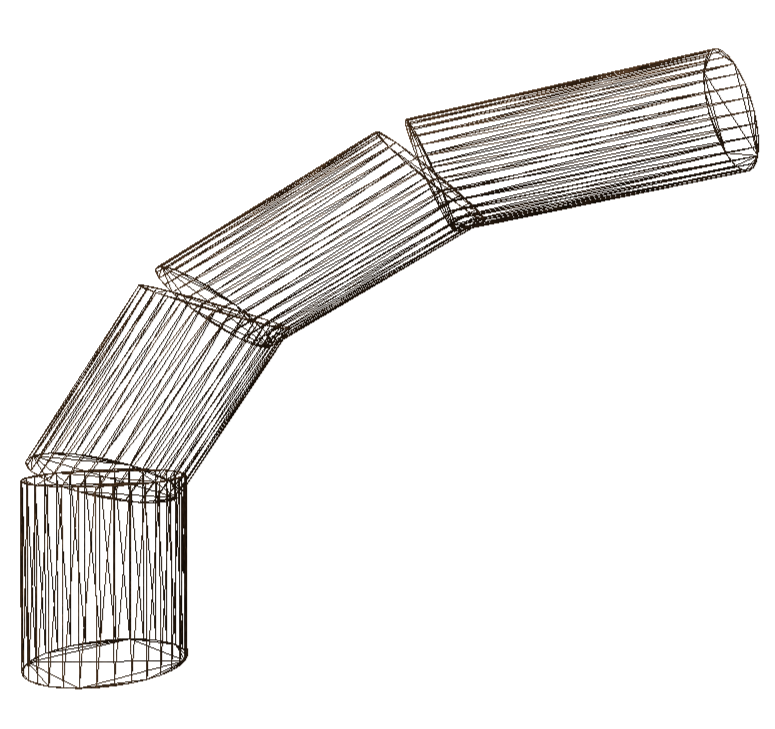
\includegraphics[scale=0.2]{Diagrams/stackedBranchesMesh.png}
		}
		\caption{Example of the continuity problem faced with stacked branching with a 25$^{\circ}$ bend per joint.}
	}
\end{figure}

\FloatBarrier

\noindent
The simple method of stacking cylinders gives an approximation of the tree structure. It is usually a good enough representation when the branch angles are not more than 25$^{\circ}$, and the size of the branches do not change. However, for a much more convincing tree structure, there will need to be a better solution. 

An improvement would be to link all of the branch segments together to make the entire branching structure seamless. The top vertices from the parent branch must be linked with the bottom of its child branch. The vertices that make up the top and bottom of a branch are circles of vertices, which are linked together using indexing. These circles will have to rotate depending on the bending direction of the branch. This means that the final model will not be made up of a large number of the same model but rather a single large model. 

There are several points to keep in mind for linked branching. The first is that this process is much less efficient than rendering the same cylindrical object many times. The reason for this is that every vertex within the tree needs to be calculated, generated, and finally linked. The second point is what happens when there are multiple branches off a single joint. This will be covered in more detail later. The final point has to do with the resolution of the branch. The resolution is the number of points making up the circumference of the branch. The resolution can be increased or decreased as needed. A higher resolution plant might look better but will also be more resource-intensive to render. Conversely, a lower resolution plant might look a bit more jagged, but be far less resource-intensive to render. An example of the linked branching can be seen below.

\begin{figure}[htbp]
	{\centering
		\vspace{7px}
		\setlength{\fboxrule}{1pt}
		\fbox{
			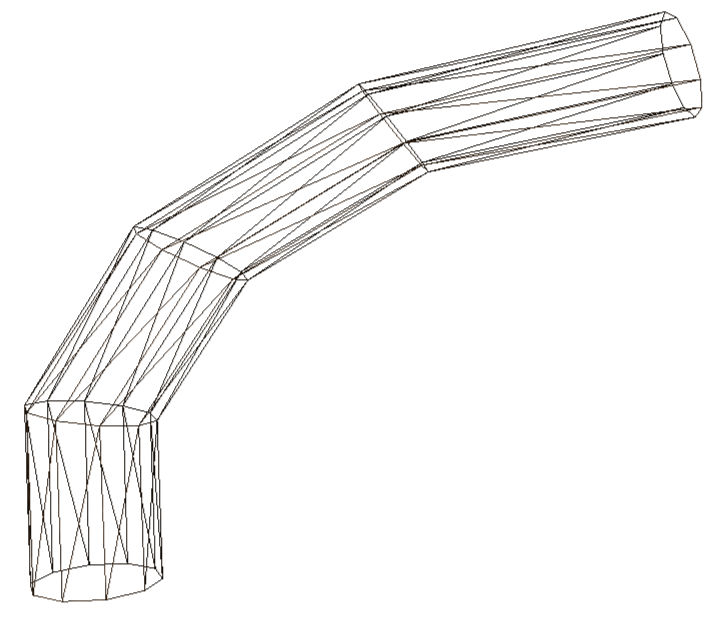
\includegraphics[scale=0.2]{Diagrams/linkedBranchesMesh.png}
		}
		\caption{Example of linked branching with a 25$^{\circ}$ bend per joint.}
	}
\end{figure}
\FloatBarrier

\noindent
This method of branch generation, at first glance, gives a very similar result to that of stacking cylinders. Although it does have a few advantages, firstly, it completely avoids the branch gap problem when there are larger angle changes, as well as branch size changes. As discussed previously, the second advantage is that the resolution is dynamic. This can be seen in figure \ref{stacked vs linked} below, where a similar-looking branch can be achieved using less than half the number of vertices, with joined branches instead of stacked branches.


\begin{figure}[htbp]
	{\centering
		\vspace{7px}
		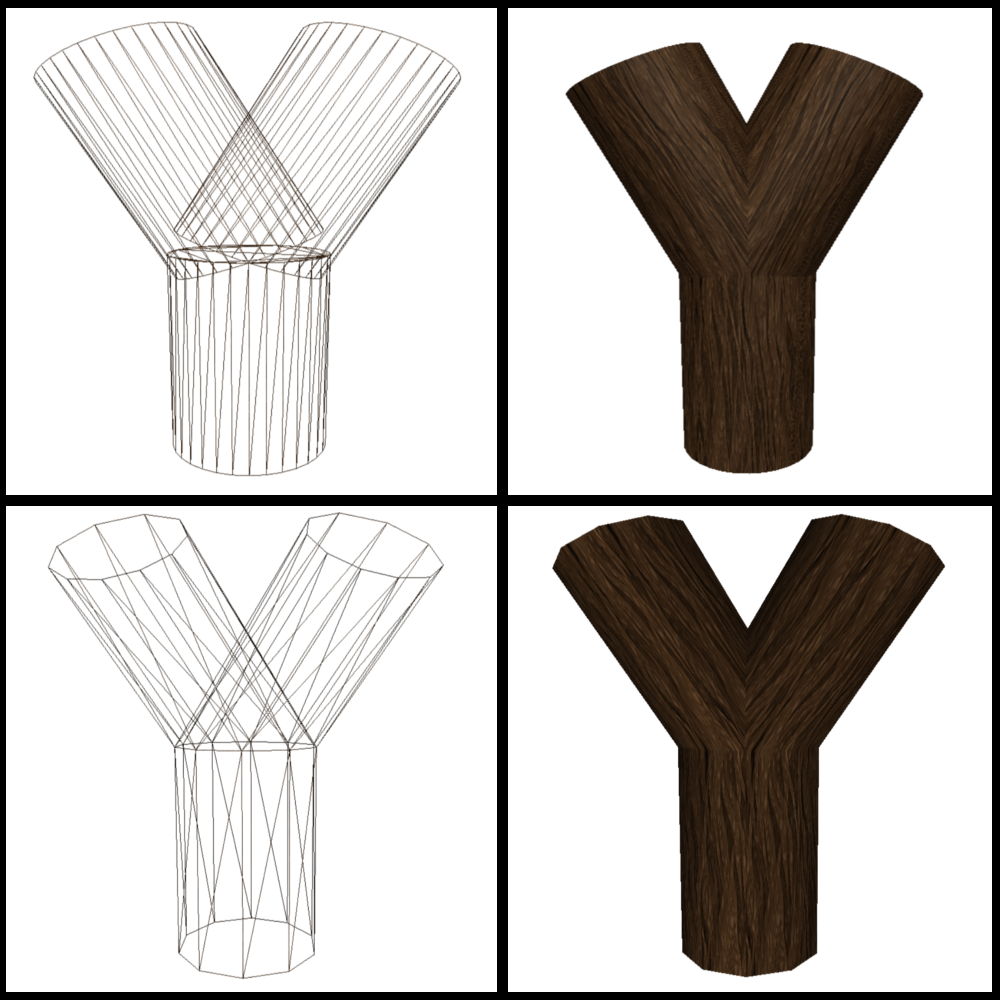
\includegraphics[scale=0.2]{Diagrams/StackedVsLinked.png}
		\caption{Diagram comparing stacked vs linked branching.}\label{stacked vs linked}
	}
\end{figure}
\FloatBarrier

\noindent
This technique of linking branches can be further improved by creating curvature from one branch to the next and by adding a smoothed noise function to the vertices that make up the branches. The advantage of this is that the branches have additional complexity and texture, which makes them look more realistic than the simple linking approach. However, the drawback is that they are more complicated to generate and more resource-demanding to render \cite{baele2005real}.

\section{Renderer}

\noindent
The renderer is the final stage in the procedural generation pipeline. It takes all of the 3D models generated by the model generator, such as leaves, branches, flowers, and renders them on the screen. \acrshort{opengl} is use used to efficiently render the models on the screen using the \acrshort{gpu}. 

The \acrshort{gpu} is a specially designed piece of hardware for processing computer graphics and image processing. It has hundreds or even thousands of individual compute cores that can be used in parallel. Due to the highly parallel nature of the \acrshort{gpu}, the \acrshort{opengl} framework helps to abstract the hardware and create an interface to interact with the \acrshort{gpu} in a more straightforward way. There are several other types of graphics \acrshort{api}, such as Vulkan, Metal, or DirectX. These \acrshort{api}s all provide a way of interacting with the hardware behind the scenes. However, each system is unique and has a different approach. Therefore, this section will not be going into great detail about the specifics of \acrshort{opengl} but rather the general concepts required for rendering the plant model on the screen. The main parts of the rendering stage have to do with how model and texture data is stored into buffer objects, and how shaders can be used to display an object on the screen.

\subsection{Models and Buffer Objects}

The model generator produces all of the information necessary for the renderer to produce the result on the screen. In general, the model data will consist of vertex data, texture coordinates, and vertex normals. The vertex data is simply the position of a point within the model, three vertices make up a face, and the faces are ultimately rendered on the screen. The texture coordinates are the locations on a texture image that maps directly to the model vertices, in order to have a textured object in the scene. Finally, the vertex normals, known as normals, are the average normal vector. A normal vector is a vector that is perpendicular to the surface at a given point and can be used for Phong shading or other types of lighting techniques.  

One of the most important parts of the rendering process is buffering the model data onto the \acrshort{gpu}. The \acrlong{vbo} (\acrshort{vbo}) is a data structure within the \acrshort{opengl} library which can be used to store this data on the \acrshort{gpu}. Generally, the data is stored as a single buffer or array with the first three values being a vertex position, the second two being a texture coordinate, and the last three being a vertex normal.

\begin{figure}[htbp]
	{\centering
		\vspace{7px}
		\setlength{\fboxrule}{1pt}
		\fbox{
			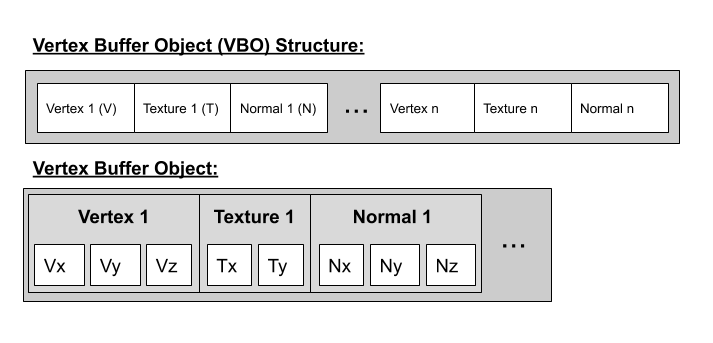
\includegraphics[scale=0.5]{Diagrams/VertexObjects.png}
		}
		\caption{Diagram showing the structure of a vertex buffer object.}
	}
\end{figure}
\FloatBarrier

\noindent
Buffer objects can be created not only for the plant branching structure but potentially for different parts of the plant, for instance, leaves or flowers. The leaves and flowers on a single tree tend to be very similar, so there is no need to have thousands of copies of a leafs' model or texture. This would be highly wasteful and unnecessary. Instead, there could be one copy of the vertex data, and texture data and instanced rendering can be used to render many copies of this single object in different places on the plant. 

\subsection{GPU Pipeline}

Modern GPU's operate very differently to a computers CPU. The GPU has hundreds if not thousands of arithmatic compute cores that operate on streams of data independantly. This is extremely useful in for graphics processing. A graphics pipeline was developed to make it easier and more efficient to compute graphics workloads. The stages of the graphics pipeline can be seen in figure \ref{graphics pipeline} below.

\begin{figure}[htbp]
	{\centering
		\vspace{7px}
		\setlength{\fboxrule}{1pt}
		\fbox{
			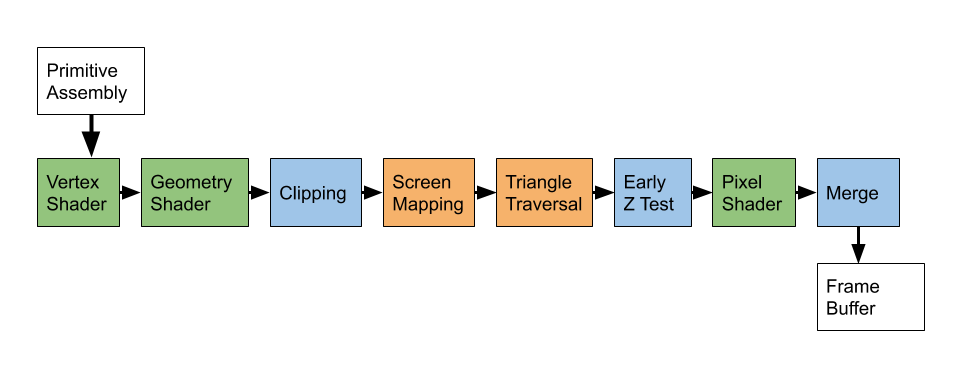
\includegraphics[scale=0.4]{Diagrams/graphicsPipeline.png}
		}
		\caption{The main stages of the rendering pipeline for a typical GPU.} \label{graphics pipeline}
	}
\end{figure}
\FloatBarrier

\noindent
Some of the stages within the graphics pipeline are programmable such as the vertex, geometry, and pixel shaders. A shader is a computer program that is used for shading an object within a 3D scene, by calculating the levels of colour and lighting for a specific part of an object within the scene. More modern types of shading can be used to provide effects like tesselation, bump mapping, and parallax mapping. Unlike the shaders, the clipping, early z-test, and merging stages are configurable but not programmable, and finally, the screen mapping and triangle traversal stages are a fixed-function stage meaning there is no way to change the functionality of these states.

The vertex shader is a fully programmable stage of processing that calculates the positions and light calculations for each vertex. The vertex is also transformed from model space to view space while applying any perspective transforms. The geometry shader is also a fully programmable stage; however, it is optional. This stage is often used to do additional calculations on entire primitives to create effects such as tessellation, complex lighting effects, or even cloth simulations. The clipping stage cuts off portions of triangles that sit on the frustum of the field of view. It is a configurable stage that is important to prevent the unnecessary per pixel calculations for triangles or parts of triangles that are out of the field of view. The fixed-function stages for screen mapping and triangle traversal firstly convert the vertices from clip space to screen space and then breaks each triangle down into fragments. Typically there is a fragment for each pixel, but with some lighting techniques, multiple fragments may be used for a single pixel. The early z-test removes fragments that are behind other fragments. This may need to be configured for specific lighting techniques. The pixel shader, also known as the fragment shader is the final programmable stage of processing. Its job is to do per-pixel calculations to determine the final colour of each pixel, taking into account textures, lighting, and other effects. Finally, the resulting fragments are merged into what will become a frame buffer.

The shader makes use of the vertex buffer data to select the color of each vertex of the plant being rendered. It does this by finding which colour is at the texture coordinate of that vertex position and then applies a lighting calculation using the vertex normal to find the amount of reflected light that is coming off the object being rendered. 


\section{Summary}

This chapter outlines the implementation of the string interpreter for representing plant-life. This consists of a three-stage process, firstly the resulting string from the rewriter is interpreted using turtle graphics to generate the skeletal structure of the plant, which is made up of joints. The model generator then uses the skeletal structure as a frame for creating the plants' branch model data. The plants' model data is finally passed to the renderer, which draws the resulting image on the screen. 

Each branch joint contains a large amount of data that is used when generating the model and is used in the physics simulator to calculate the motion of each branch, which will be covered in more detail in chapter \ref{physics chapter}. The way that the model generator creates its geometry can easily be changed or improved to generate more complex branch models. 

The renderer uses the model data, such as vertices, textures, and normals, and stores these in GPU memory in the form of buffer objects. A graphics rendering pipeline is used with programmable shaders to calculate light and other effects to generate the resulting image of the plant on the screen. 

Using a skeleton representation for the tree has the advantage that the model generator and the renderer work independantly of the representation. Both the model generator and renderer can be improved without having to modify the turtle graphics interpreter or the skeletal structure. This also means that the physics simulation is independant of the model generator, as the skeletal joints will be manipulated effecting the geometry of the plant model only after the model has been generated. 






